\chapter{System Analysis}
\section{Module Description}
The Budgetbeam platform is strategically divided into functional modules:
\begin{itemize}
    \item \textbf{Authentication \& Profile Module:} Manages secure user identities, session persistence, and personal preferences using Laravel's robust authentication middleware.
    \item \textbf{Budget Management Module:} Serves as the navigational hub for the user, allowing for the definition of time-bound financial limits across various categories such as Rent, Groceries, and Education.
    \item \textbf{Expense Tracking Module:} The core transactional engine of the application, enabling the seamless logging of daily expenditures with automatic association to budgets and categories.
    \item \textbf{Analytics \& Reporting Module:} Leverages Chart.js to provide users with a visual breakdown of their spending habits, remaining balances, and savings metrics in real-time.
\end{itemize}

\section{Business Rules}
\begin{itemize}
    \item \textbf{Transaction Integrity:} Every expense must be associated with a valid user\_id and a category\_id.
    \item \textbf{Budget Constraints:} Users are alerted visually when their expenditure for a specific category exceeds $90\%$ of its allocated budget.
    \item \textbf{Privacy Protocols:} No user can view or modify the financial records of another user; all queries are strictly scoped to the authenticated session.
    \item \textbf{Categorization:} Expenses logged without a specific category are automatically funneled into a 'General' catch-all category to prevent data loss.
\end{itemize}

\section{Use Case Model}
\subsection{Use Case Descriptions}
\begin{longtable}{|l|l|p{8cm}|}
\caption{Use Case Descriptions for Budgetbeam} \\
\hline
\textbf{ID} & \textbf{Use Case} & \textbf{Description} \\ \hline
UC01 & Register / Login & The user creates a new account or authenticates with existing credentials. \\ \hline
UC02 & Manage Budgets & The user adds, edits, or removes financial limits for specific categories. \\ \hline
UC03 & Record Expense & The user logs a new expenditure with details on amount, date, and category. \\ \hline
UC04 & View Analytics & The user views charts and summaries of their total spending vs budget. \\ \hline
UC05 & Export Report & The user generates a PDF/CSV summary of their monthly financial activity. \\ \hline
UC06 & Manage Categories & The user creates custom categories for more granular tracking. \\ \hline
\end{longtable}

\subsection{Use Case Diagram}
\begin{figure}[h!]
    \centering
    \caption{Use Case Diagram for Budgetbeam}
    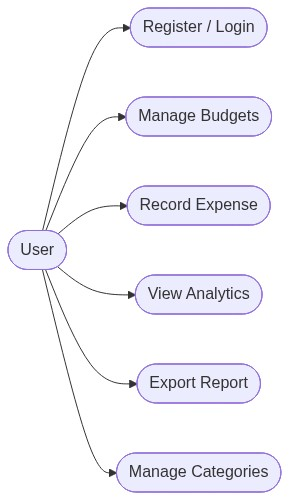
\includegraphics[width=0.9\textwidth]{use_case.png}
\end{figure}

\section{Feasibility Analysis}
\subsection{Technical Feasibility}
The tech stack for Budgetbeam is highly feasible. PHP 8.2 with Laravel provides built-in authentication, ORM, and routing which simplifies development. PostgreSQL ensures high-performance relational storage.
\subsection{Economical Feasibility}
The project relies on open-source technologies, eliminating licensing costs. Hosting a Laravel application on standard cloud infrastructures is cost-effective and scalable.
\subsection{Operational Feasibility}
The intuitive UI and automated tracking features reduce cognitive load for users, making the task of personal budgeting friction-free and sustainable for long-term use.

\section{Actors and Roles}
\textbf{User (Primary Actor):} The sole actor within Budgetbeam. They own their data, manage their budgets, and analyze their own financial reports.

\section{Activity Diagram}
\begin{figure}[h!]
    \centering
    \caption{Activity Diagram for Budgetbeam platform}
    
\includegraphics[width=0.9\textwidth]{activity.png}
\end{figure}
